\subsection{Research}				% Bitte subsection statt section nutzen
%\subsubsection{Research}		% wenn subsection noetig, bitte subsubsection
In the beginning I had problems finding the time to become acquainted with the code base of the Realtime Football Analysis Tool, so I concentrated on different tasks for the project. The obvious choice was doing research to collect information other team members work could base upon.

\subsubsection{Flask research}
The first thing I did, was filter the Flask man pages for all the pages relevant to our project. As the Flask documentation is quite extensive I used ChatGPT for this task. Admittedly, this does not show any work from my side worth mentioning, but I wanted to include it anyways as this might make future research regarding Flask easier. The result of ChatGPTs hard work can be found in the project folder and is called "flask\_imports\_doc.txt".

\subsubsection{Research for Football penalty catalog}
One goal of this project group was expanding the capabilities of the Realtime Football Analysis Tool to record penalties and their consequences. For this I researched all the penalties possible in the National Football League (NFL) and condensed them into a document. Then it was pointed out to me, that German Football Rules were not based on the rule set of the NFL but instead on the more detailed and less dangerous to play rule set of the National Collegiate Athletic Association (NCAA). To correct this some rules had to be adjusted and a lot of small rules had to be added, but in the grand scheme of things both rule sets are very similar. 


\subsection{Programming}
\subsubsection{Show play type in Drive List}
The problem with the game page at its current state was, that in the drives did now show their play type. This made it quite hard having an overview who has the drive during a game. My straightforward solution was showing the play type on each entry in the drive list. The final result in shown below.\\ \\
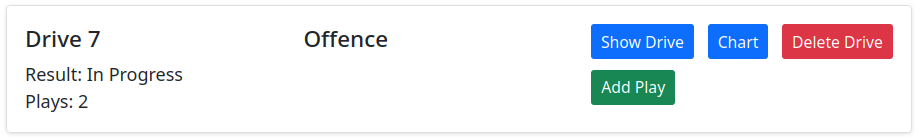
\includegraphics[width=\textwidth]{Drive_list_button.png} \\
For the play type to show up in the 

\begin{minted}{python}
@@ -66,6 +66,9 @@ class GameController:
	
	@login_required
	def game_detail(self, game_id: int) -> str:
		game = GameModel.get_by_id(game_id)
+       for drive in game.drives:
+            if len(drive.plays) > 0:
+                print(drive.plays[0].odk)
		return render_template(template_name_or_list='game/game_detail.html', game=game)
\end{minted}

\begin{minted}{python}
@@ -31,7 +31,7 @@ class PlayController:
	
			options = self._get_add_play_form_options()
			play = PlayModel.query.get_or_404(play_id)
-
+       	drive = DriveModel.query.get_or_404(play.drive_id)
			if request.method == 'POST':
				try:
					result_form = request.form.get('result')
\end{minted}

\begin{minted}{python}
@@ -67,6 +67,7 @@ class PlayController:

		return render_template('play/add_play.html',
								play=play,
+                               drive=drive,
								options=options,
								drive_id=play.drive_id)	
\end{minted}	

\begin{minted}{html}
@@ -41,6 +41,18 @@
			<div class="card-body">
				<div class="d-flex justify-content-between align-items-start">
				<h5 class="card-title">Drive {{ loop.revindex }}</h5>
+                
+                    
+                        <h5 class="card-title">Offence</h5>
+                    
+                        <h5 class="card-title">Defence</h5>
+                    
+                        <h5 class="card-title">Special</h5>
+                    
+                        <h5 class="card-title">Unknown play type: {{ drive.plays[0].odk }}</h5>
+                    
+
+                

					<div>
						<a href="{{ url_for('drive_play_chart', game_id=game.id, drive_id=drive.id) }}" class="btn btn-sm btn-primary">Chart</a>	
\end{minted}

\subsubsection{Add Play button in Drive List}
My next story point was the inclusion of the Add Play button on the drive list entry, which was an area of expertise I was already accustomed to. The play button was already shown in the last paragraph, but here it is one more time:\\ \\
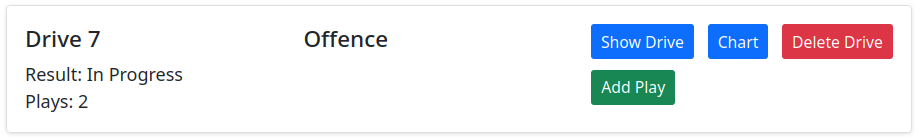
\includegraphics[width=\textwidth]{Drive_list_button.png} \\


\begin{minted}{python}
	
\end{minted}



\begin{minted}{python}
	
\end{minted}


\subsubsection{Small fixes}


\begin{minted}{html}
@@ -4,8 +4,8 @@
 
 <div class="row mb-4">
	<div class="col">
-        <h2>{{ game.game_name }}</h2>
-        <p>{{ game.date.strftime('%Y-%m-%d') }} {{ game.time }}</p>
+        <h2>{{ game.name }}</h2>
+        <p>{{ game.date.strftime('%d.%m.%Y') }} {{ game.time }}</p>
	</div>
	<div class="col text-end">
		<a href="{{ url_for('drive_chart', game_id=game.id) }}" class="btn btn-primary">Show Drive Chart</a>
\end{minted}



\subsection{Visual Design}


